\documentclass[../main.tex]{subfiles}
\graphicspath{ {\subfix{../../img/}} }

\begin{document}
\section{Application and Results}

    \subsection{\textit{V\textsubscript{GS}--I\textsubscript{D}} Characteristics of N-Channel MOSFET}
        \begin{figure}[H]\centering
            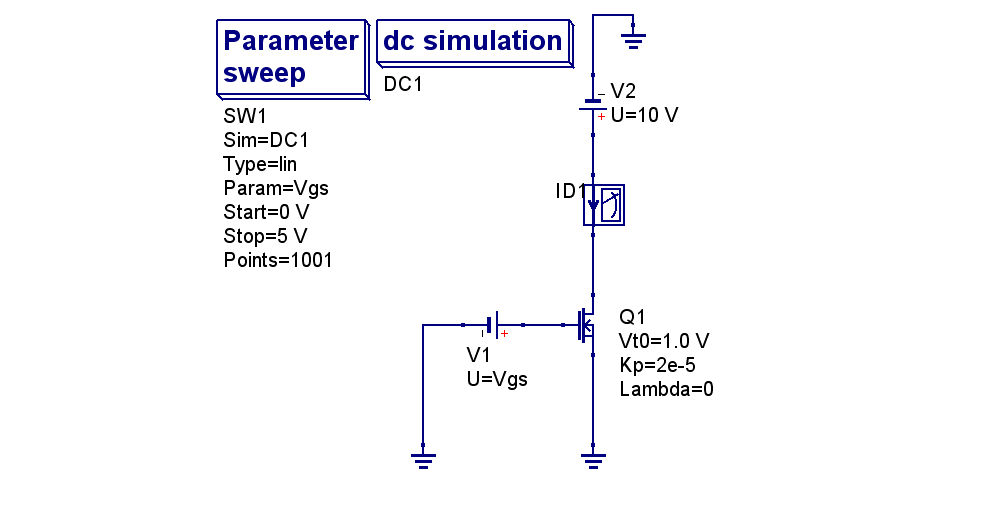
\includegraphics[width=\textwidth]{p1.sch.png}
            \caption{Experiment circuit for gate characteristic}\label{fig:p1.sch}
        \end{figure}

        To observe $V_{GS}-I_D$ characteristic of a n-channel MOSFET, the circuit as depicted above is 
        constructed in QUCS. Under constant drain to source voltage $V_{DS}=\SI{10}{\volt}$, gate to source
        voltage $V_{GS}$ is swept from \SI{0}{\volt} to \SI{5}{\volt}. During which the drain current $I_D$ 
        is measured. The following graph is created by plotting $I_D$ against $V_{GS}$.

        \begin{figure}[H]\centering
            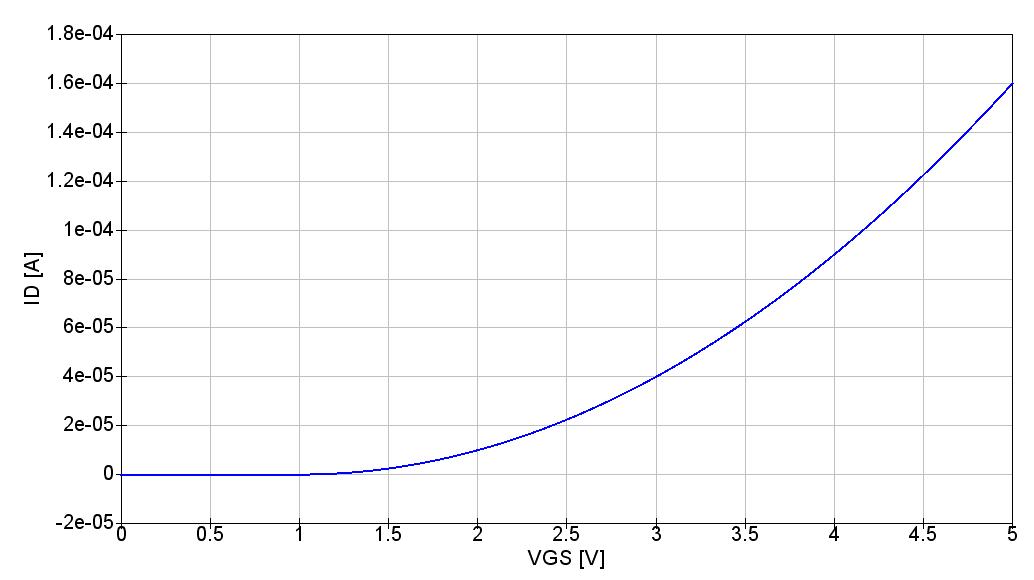
\includegraphics[width=\textwidth]{p1.gph.png}
            \caption{$V_{GS}-I_D$ characteristic graph}\label{fig:p1.gph}
        \end{figure}

        Notice that the simulation settings ensure that $V_D \geq V_{GS}-V_t$, so that the transistor remains 
        saturated during the entire sweep. Since the expression for the drain current in this mode of operation is 
        \begin{equation*}
            I_D = 
            \begin{cases}
                0 &V_{GS} < V_{th} \\
                \frac{1}{2} \kappa (V_{GS}-V_{th})^2 &V_{GS} \geq V_{th}                
            \end{cases}
            \qquad \kappa \triangleq \mu_{n}C_{ox}\frac{W}{L_{eff}}         
        \end{equation*}
        the graph is expected to be half of a parabola. Which is the case. It also can be seen from the graph that 
        the drain current remains effectively 0 until the gate voltage surpasses the threshold voltage, in this 
        case, \SI{1}{\volt}.

        \begin{table}[H] \centering
            \begin{tabular}{|c||c|c|}
                \hline
                $V_{GS}$ [\SI{}{\volt}] & Calculated [\SI{}{\micro\ampere}] & Simulation [\SI{}{\micro\ampere}] \\
                \hline
                \hline  $1$     &$0$     &    $3.97\texttt{e-12}$    \\
                \hline  $2$    &$10$    &    $10$    \\
                \hline  $3$    &$40$    &    $40$    \\
                \hline  $3$    &$90$    &    $90$    \\
                \hline  $5$   &$160$   &    $160$    \\
                \hline
            \end{tabular} \caption{Comparison of calculated values and simulation results} \label{tab:comp_Vgs_Id}
            \end{table}
        
        Simulation results agreed with calculations to 7 significant digits.


    \subsection{\textit{V\textsubscript{DS}--I\textsubscript{D}} Characteristics of N-Channel MOSFET}
        \begin{figure}[H]\centering
            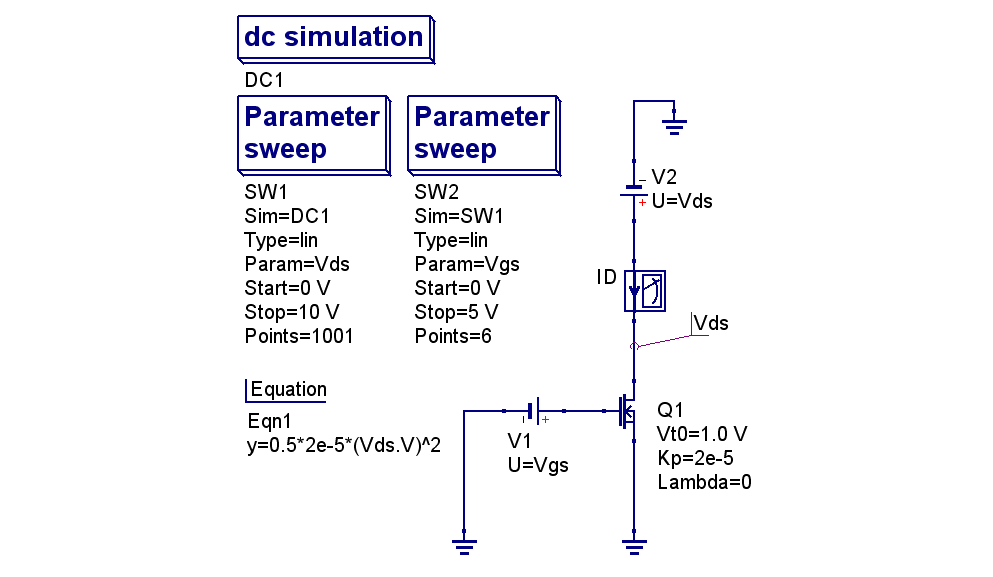
\includegraphics[width=\textwidth]{p2.sch.png}
            \caption{Circuit}\label{fig:p2.sch}
        \end{figure}

        To observe the $V_{DS}-I_D$ characteristics, experiment setup is changed by adding another parameter 
        sweep for sweeping the drain voltage. Gate voltage sweep discretised and varied between 0 and \SI{5}{\volt}
        with \SI{1}{\volt} increments. $I_D$ current is measured.
        
        Family of drain current curves are plotted against $V_{DS}$ and each one labelled.\footnote{Apart from V\textsubscript{GS}=\{0,1\} V since the plot doesn't allow to mark them seperately.}
        The parabola $i=\frac{1}{2}\kappa(V_{DS})^2$ is also plotted with dashed black curve.
        
        Simulation results again agree with theoratical calculations to 7 significant digits.

        \begin{figure}[H]\centering
            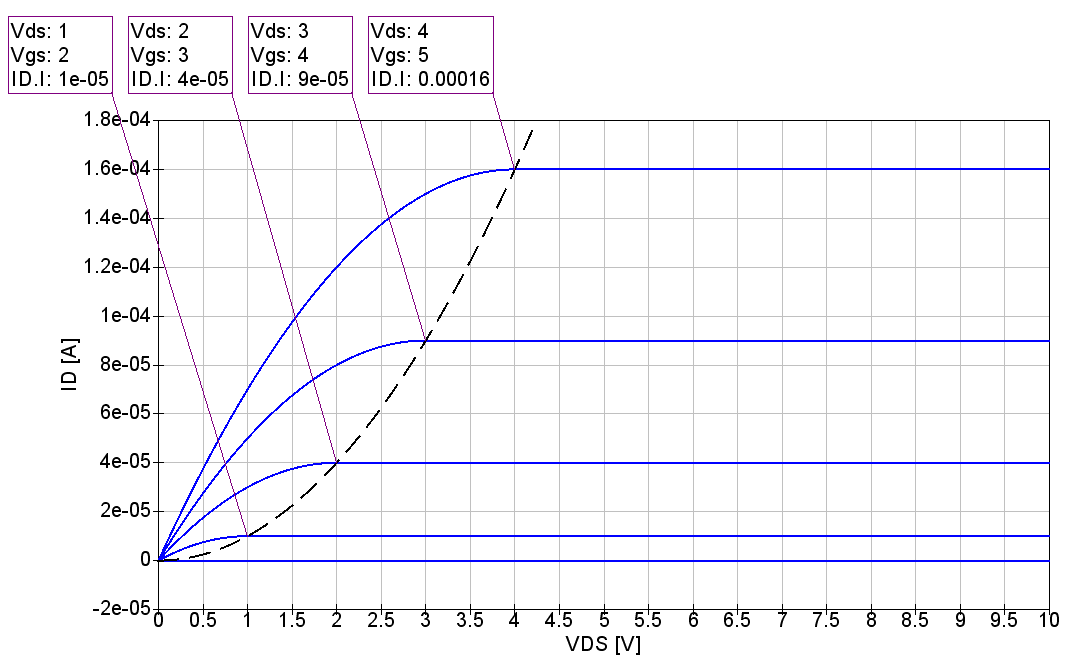
\includegraphics[width=\textwidth]{p2.gph.png}
            \caption{graph}\label{fig:p2.gph}
        \end{figure}

        As expected, for any gate voltage that doesn't put the transistor in cut-off, as $V_{DS}$ increases, drain current 
        starts more or less linear, eventually bending to form a downward looking parabola, and finally at the point
        $V_{DS}=(V_{GS}-V_{th})$, transistor saturates and $I_D$ remains constant, independent of the $V_{DS}$. 
        Increase in $V_{GS}$ increases both the $V_{DS}$ that saturates the transistor, and the $I_D$ that flows
        when it saturates. 

        For $V_{GS}=\SI{0}{\volt}$ and $V_{GS}=\SI{1}{\volt}$, the drain current remains 0. Transistor is in cut-off
        region, since the electric field at the gate is lacking or not sufficient enough to form an inversion layer 
        on the channel region. Since the structure of the MOSFET is so that there are two P-N junctions between 
        drain and source with opposite directions, if a channel is not formed, there is a reverse biased P-N junction
        between drain and source for either polarity of the $V_{DS}$, hence no current can flow between drain and source.

    \pagebreak


    \subsection{Effect of Series Gate Resistor}
        In this part, a \SI{1}{\kilo\ohm} resistor is introduced in series with the gate, to observe its 
        effect on the $V_{DS}-I_D$ plot of the previous stage. Since gate of a MOSFET \textit{draws no current},
        this resistor appears completely irrelevant. And indeed, $V_{DS}-I_D$ plot in this setting is completely 
        identical to that of previous stage. To avoid duplicating the entire stage, this barely modified 
        schematic and the identical plot are not given seperately.

        This gate resistor, however, starts doing interesting things, if looked correcty. By correctly, we mean, 
        in time domain. Here, the circuit is carried into a transient simulation, with a relatively high frequency
        square wave of magnitude \SI{5}{\volt} applied to the gate, with the \SI{1}{\kilo\ohm} series resistor.
        However, since default parameters for the MOSFETs in QUCS apparently choosen so that the transistor 
        is quite close to ideal\footnotemark, MOSFET is replaced by a real small signal discrete MOSFET, BSS123, that 
        happens to be in QUCS library.
        \footnotetext{And there are way too many different capacitance parameters, and I wasn't sure what a realistic value would be anyway.}

        \begin{figure}[H]\centering
            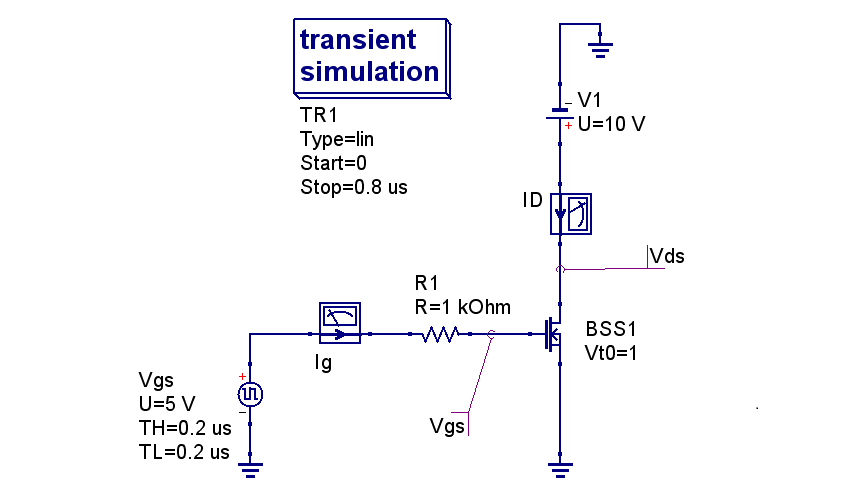
\includegraphics[width=\textwidth]{p2.2.sch.png}
            \caption{Transient simulation to see effect of series gate resistor.}\label{fig:p2.2.sch}
        \end{figure}

        \begin{figure}[H]\centering
            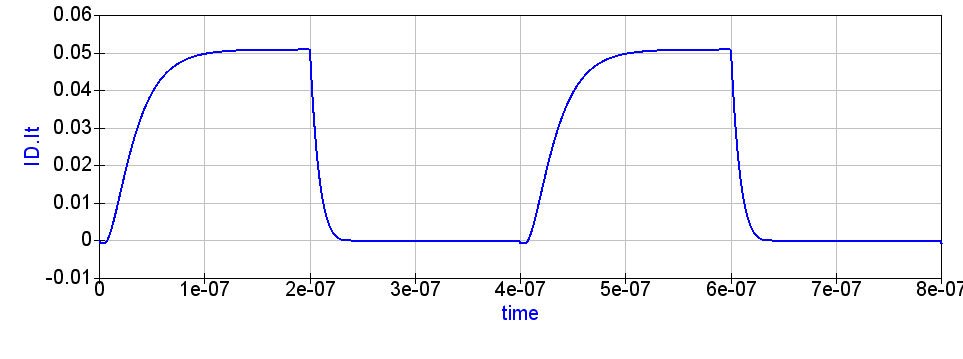
\includegraphics[width=\textwidth]{p2.2.gph2.png}
            \caption{}\label{fig:p2.2.gph}
        \end{figure}

        As a result, the drain current starts to behave awkwardly. 
        Values, of course are different since the transistor is different, but what matters is the shape of the
        waveform, it looks \textit{almost like capacitor charge-discharge pattern}. Indeed, if the voltage 
        and the current at the gate were to be measured, we see the following graph.

        \begin{figure}[H]\centering
            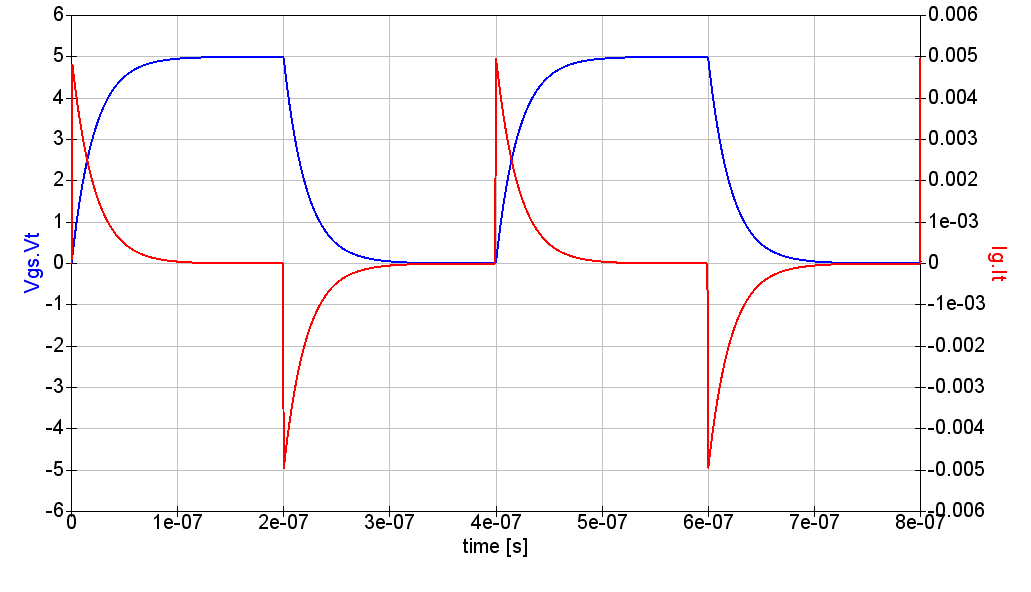
\includegraphics[width=\textwidth]{p2.2.gph.png}
            \caption{}\label{fig:p2.2.gph2}
        \end{figure}

        \pagebreak
        The capacitive response of the gate can clearly be seen from this graph. Of course
        gate behaves capacitor-like, since the gate plate and the bulk effectively forms a capacitor. 
        Since the gate pretty much fully charges at about \SI{100}{\nano\second}, assuming this is 
        roughly equal to $5 \tau$, the approximate capacitance of the gate can be calculated.
        \begin{equation*}\begin{aligned}
            5\tau &\approx 100\times 10^-9 \texttt{s}\\
            \tau &= RC \approx \SI{20}{\nano\second}, \quad R=\SI{1}{\kilo\ohm}\\
            &\implies C \approx \SI{20}{\pico\farad}\\
        \end{aligned}\end{equation*}

        Therefore, the gate capacitance of this MOSFET should be around at the order of \SI{20}{\pico\farad}'s  
        Another interesting observation is that during the transitions of the applied gate voltage, the gate momentarily draws 
        around \SI{5}{\milli\ampere} of current!\footnote{At least this for this transistor.} That's 
        quite a lot of current to be drawn by something supposed to draw no current.  
        \pagebreak

        
    \subsection{Effect of Negative $V_{GS}$}
        What follows that is the case when a negative $V_{GS}$ is applied to the gate. Then, the electric field between 
        the gate plate and the body not only isn't sufficient to pull electrons into the channel region and create a 
        channel, but it pushes the electrons away, not allowing any current to flow between drain and source. While 
        it is not necessary for enhancement type NMOS' to apply a negative gate voltage, it can help discharging the 
        gate more quickly and hence allow the transistor to fall into cut-off mode more abruptly.

        Following is another test setup, where the same circuit as before is not first driven with \SI{5}{\volt} positive 
        pulse, and then with $\pm\SI{5}{\volt}$ symmetric pulse.

        \begin{figure}[H]\centering
            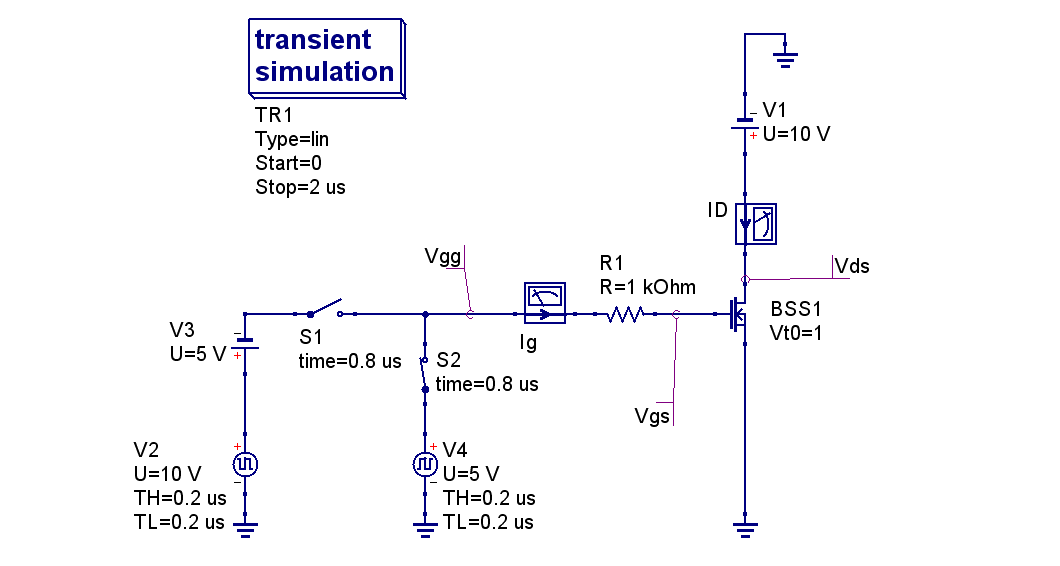
\includegraphics[width=\textwidth]{p2.3.sch.png}
            \caption{}\label{fig:p2.3.sch}
        \end{figure}

        As expected, applying a negative voltage to a charged gate increased the speed of its discharge, thus decreasing 
        the fall time of the drain current. However, now it takes proportionally longer to charge the gate above the 
        threshold, thus delaying the rise of the drain current.

        \begin{figure}[H]\centering
            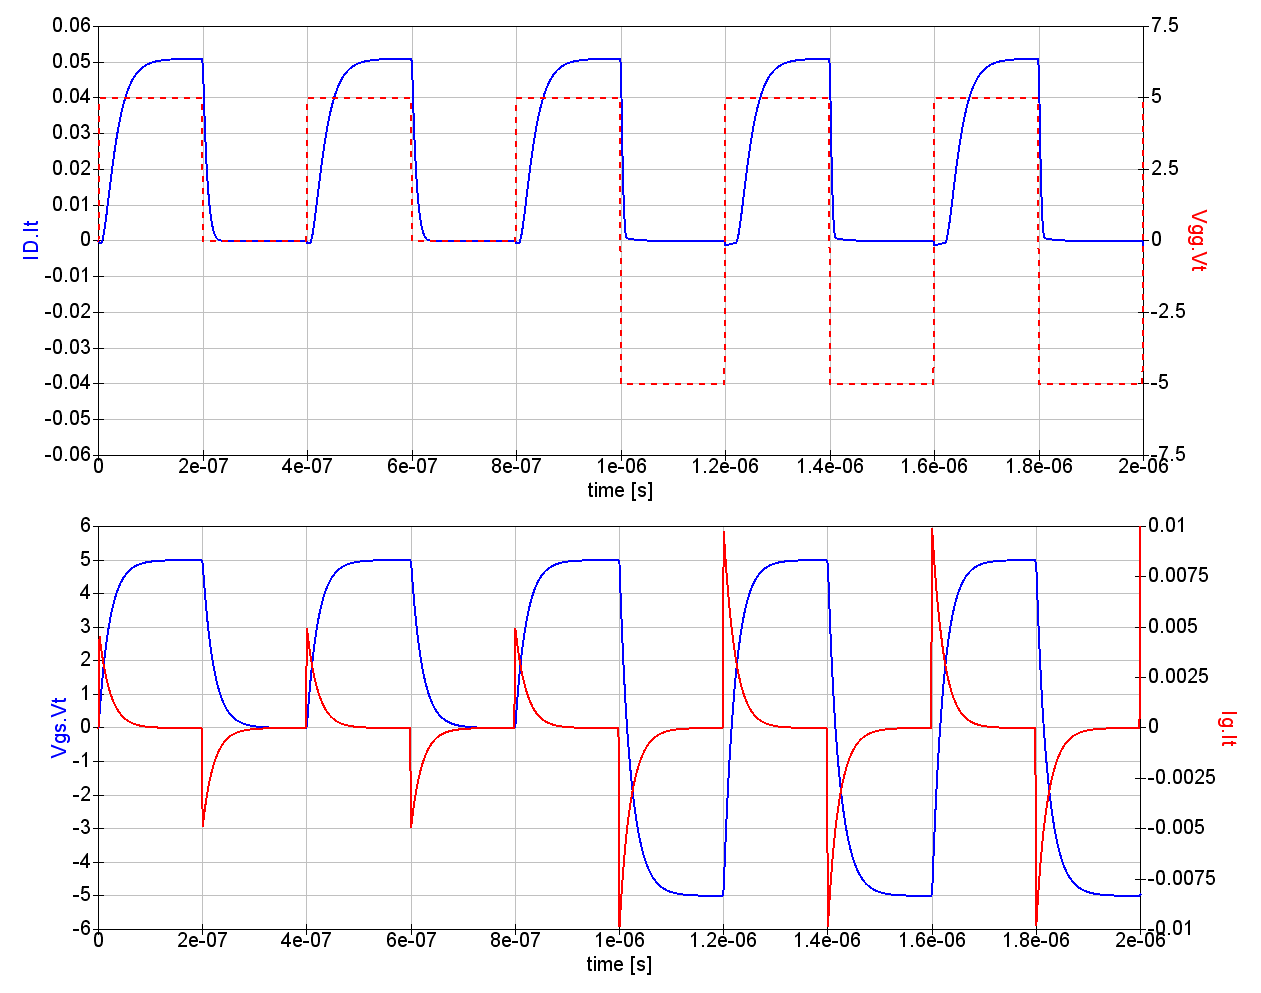
\includegraphics[width=\textwidth]{p2.3.gph.png}
            \caption{ \\Top: Drain current (left), applied gate voltage (right)\\
                        Bottom: Gate current (left), gate voltage (right) }\label{fig:p2.3.gph}
        \end{figure}

        

\end{document}